\documentclass{beamer}


% PACKAGES==========================================================================================
\usepackage{hyperref}
\usetheme[hideothersubsections]{PaloAlto}
\useinnertheme{rectangles}
\usecolortheme{beaver}
\usepackage[version=3]{mhchem}
\usepackage{caption}
\usepackage{textpos}
\usepackage{amsmath}
\usepackage{etoolbox}
\usepackage{wrapfig}
\usepackage{multicol}
\usepackage[caption=false]{subfig}
\usepackage[font=small,skip=0pt]{caption}



% SETTINGS==========================================================================================
\setbeamerfont{caption}{series=\normalfont,size=\fontsize{5}{5}}
\setbeamercolor{section in sidebar}{fg=darkgray}            %color of the active section
\setbeamercolor{section in sidebar shaded}{fg=lightgray}     %color of the inactive section
\setbeamercolor{subsection in sidebar}{fg=darkred}         %color of the active subsection
\setbeamercolor{subsection in sidebar shaded}{fg=lightgray}  %color of the inactive subsection
%\setbeamercolor{title in sidebar}{fg=...}              %color of the presentation title
%\setbeamercolor{author in sidebar}{fg=...}             %color of the author  
\setbeamertemplate{section in toc shaded}[default][10]
 
\setbeamerfont{block body}{size=\tiny}
%\setbeamertemplate{blocks}[square][shadow=false]
\setbeamertemplate{blocks}[default]
\setbeamertemplate{bibliography item}[text]
\setlength{\parindent}{0pt}
\setbeamertemplate{caption}[numbered]


\defbeamertemplate*{section in toc}{my theme}
{\leavevmode\leftskip=0.5em\large{\usebeamercolor[fg=darkred]{titlelike}\inserttocsectionnumber.} \inserttocsection\par}

\defbeamertemplate*{subsection in toc}{my theme}
{\leavevmode\leftskip=0.5em\normalsize{\usebeamercolor[fg=darkgray]{titlelike}\inserttocsectionnumber.\inserttocsubsectionnumber.} \inserttocsubsection\par}



% Define footer
\setbeamertemplate{footline}{bg=primary}
\makeatother
\setbeamertemplate{footline}
{
    \leavevmode%
    \hbox{%
    \begin{beamercolorbox}[wd=.4\paperwidth,ht=2.25ex,dp=1ex,center]{author in head/foot}%
       \usebeamerfont{author in head/foot}\insertshortauthor\ (Chris Ngigi - DEC I)
    \end{beamercolorbox}%
    
    \begin{beamercolorbox}[wd=.4\paperwidth,ht=2.25ex,dp=1ex,center]{title in head/foot}%
        \usebeamerfont{title in head/foot}\insertshorttitle
        \hfill
    \end{beamercolorbox}    
        
    \begin{beamercolorbox}[wd=.2\paperwidth,ht=2.25ex,dp=1ex,center]{title in head/foot}%
        \usebeamerfont{title in head/foot}
        \hfill    
        \hspace{2em}\insertframenumber/\inserttotalframenumber
    \end{beamercolorbox}}%
}

\beamertemplatenavigationsymbolsempty  % disable navigation
\setbeamertemplate{sidebar}{%
   \vspace*{0cm}
    \vspace*{\fill}
   \vspace*{0.1cm}
   \setbeamersize{sidebar width left=2cm}
   
\includegraphics[width=0.55cm]{./figs/utias_logo_blue.jpg}
}
    
\setbeamerfont{section number projected}{family=\rmfamily,series=\bfseries}
\setbeamercolor{section number projected}{bg=lightgray,fg=darkred}
\setbeamertemplate{sections/subsections in toc}[square]

\addtobeamertemplate{frametitle}{}{%
\begin{textblock*}{1cm}(-1.8cm,-1.2cm)

\includegraphics[height=1cm,width=1cm]{./figs/utias-logo2.jpg}
\end{textblock*}}

\makeatletter
\patchcmd{\beamer@sectionintoc}{\vskip1.5em}{\vskip0.5em}{}{}
\patchcmd\insertverticalnavigation{\dohead}{\vskip-35pt\dohead}{}{}
\makeatother


% ==================================================================
% NOW MAIN DOCUMENT

%%========================================================================

\title[]{Development of h-p Adjoint-based error estimation for LES of reactive flows }
\author[]{{Christopher Ngigi \texorpdfstring{\\ \tiny{Ph.D. Pre-Candidate} \\} \footnotesize Supervisor: Prof. C. P. T. Groth}}
\titlegraphic{
\includegraphics[width=0.15\textheight]{./figs/utias_logo_blue.jpg}}
\institute[]{Doctoral Examination Committee \\ Meeting I \\ University of Toronto, Institute for Aerospace Studies}
\date[]{April 6, 2015}
	
%%========================================================================

\begin{document}

\addtocounter{framenumber}{-1}
\begingroup
\makeatletter
\setlength{\hoffset}{-.5\beamer@sidebarwidth}
\makeatother
\begin{frame}[plain]
    \titlepage	
\end{frame}

%==========================================================================================
\begin{frame}[plain,c]
\begin{minipage}[t][1\textheight]{0.9\textwidth}
\begin{alertblock}{\large{Outline: }}
\small

\tableofcontents[hideallsubsections]

\end{alertblock}
\end{minipage}
\end{frame}
\endgroup

%===========================================================================================

% this section adds a mini TOC between sections. CTRL+U to activate
%\AtBeginSection[]
%{
%     \begin{frame}[plain,c]
%     \begin{minipage}[t][1\textheight]{0.8\textwidth}
%     %\setbeamercolor{section in toc shaded}{use=structure,fg=lightgray}
%     \setbeamercolor{section in toc}{fg=darkred}
%     \setbeamercolor{subsection in toc}{fg=darkgray}
%          
%     %
\includegraphics[width=1.5cm]{./figs/utias_logo_blue.jpg}
%     \begin{alertblock}{\large{Section:}}
%     \tiny
%     \tableofcontents[currentsection, sectionstyle=show/shaded, subsectionstyle=show/show/hide]
%     \end{alertblock}
%     \end{minipage}
%     \end{frame}
%}

%==========================================================================

\section{Introduction}
\subsection{Computing power}
\begin{frame}%[allowframebreaks]
\frametitle{Introduction}
\vspace{-6pt}
\scriptsize 
Cost of experiment vs numerical simulation
\begin{itemize}
\tiny
\item Computational Fluid Dynamics (CFD) developed to reduce the time and cost of prototypes in fluid flow experiments. 
\item Complexities may be expensive to set up in experimental modeling
\item CFD methods and models have been developed to capture this phenomenon to varying extents of accuracy
\end{itemize}
Moore's law: Computing power $\approx$ doubles every 2 years
\vspace{-1mm}
\begin{figure}[h!]
%\centering
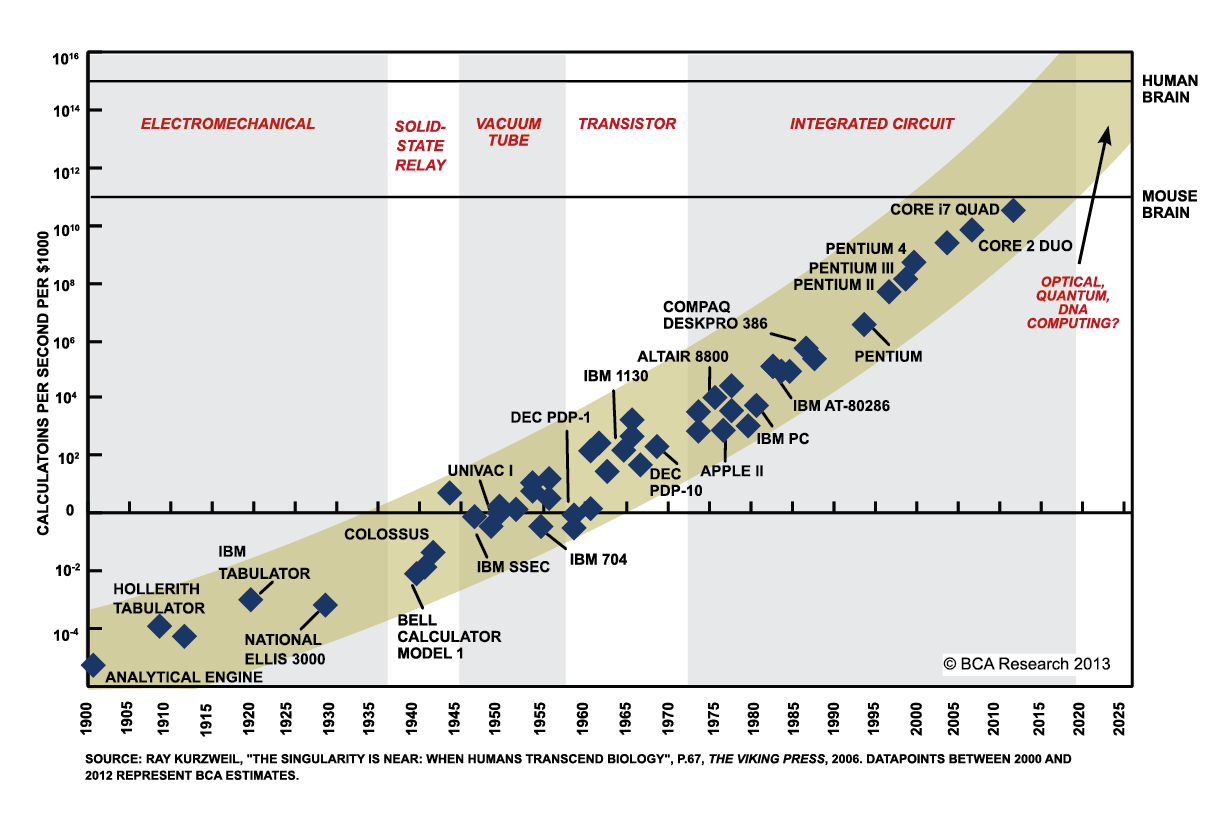
\includegraphics[height=0.47\textwidth, trim=0cm 1.2cm 0 1.2cm,clip=true]{./figs/MooresLaw.png}
\caption{Moore's Law over the years [BCA Blog] \cite{MooreLaw}]}
\label{fig:Moore}
\end{figure}
\end{frame}

%==========================================================================

\subsection{Turbulent combustion - experimental}
\begin{frame}%[allowframebreaks]
\frametitle{Turbulent combustion - experimental}
\small{Turbulent combustion: real fluid flows almost always involve turbulence. Large eddy simulation (LES) - technique to achieve higher accuracy than Reynolds' averaged Navier Stokes (RANS) at lower computational cost (time, resources) than direct numerical simulation (DNS).}
\begin{minipage}[0.5\textheight]{\textwidth}
\begin{columns}[T]
\begin{column}{0.65\textwidth}
\vspace{20pt}
\small{Lifted turbulent Ethylene ($C_2H_4$) jet flame issuing into a concentric co-flow of air. Zone between flame-base and nozzle may have partial premixing. Fuel and air temperature, pressure near standard [K{\"o}hler 2006] \cite{Kohler}}
\begin{itemize}%[<+->]
\tiny
\setlength\itemsep{-0.7mm}
\item Dimensions: Nozzle diameter = 2.0 mm; Co-flow air annulus diameter = 140 mm\\
\item Exit Reynolds number: 10000
\item Air mass flow: 320 g/min 
\item Mean fuel jet velocity: 44 m/s 
\end{itemize}
\end{column}

\begin{column}{0.3\textwidth}
\vspace{0pt}
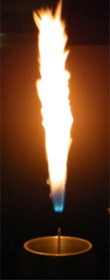
\includegraphics[height=1.4\textwidth]{./figs/dlrflame.png}
\newline
\tiny
[K{\"o}hler 2006] \cite{AdelaideISF}
\end{column}
\end{columns}
\end{minipage}
\end{frame}

%==========================================================================

\subsection{Turbulent combustion - simulation}
\begin{frame}%[allowframebreaks]
\frametitle{Turbulent combustion - simulation example}
\scriptsize
{Considering that DNS resolves all the scales, LES models sub-filter scales (SFS) while resolving the larger scales, and that RANS models all the scales, then we can expect the most accurate to be DNS, then LES, then RANS. Computational results that Yang, Pope and Chen  obtained are:}
\vspace{-25pt}
\begin{figure}
\label{fig:DNSLES}
\centering
\subfloat[\tiny{temperature in x-y plane: DNS (l), LES/PDF (r)} \label{fig:contourDNS}]{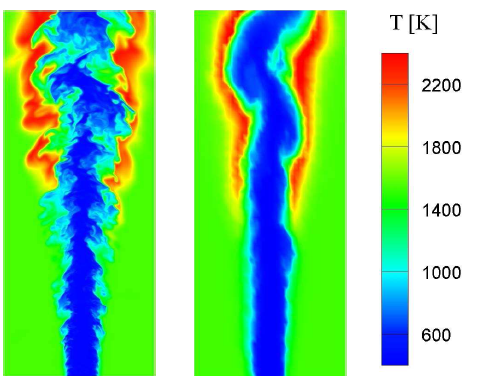
\includegraphics[width=0.7\textheight]{./figs/Temperatures.png}}
\subfloat[\tiny{Mean temperature :DNS and LES} \label{fig:meanTemp}]
{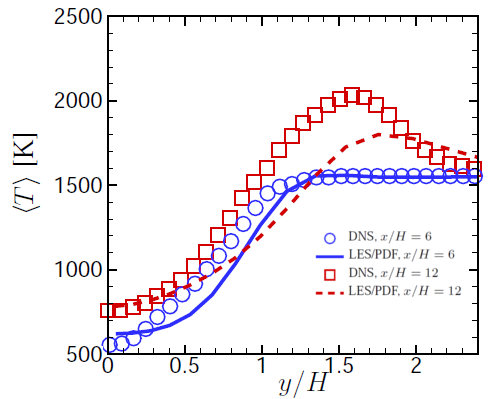
\includegraphics[width=0.65\textheight]{./figs/Temp_DNS_LES2.png}}
\tiny{\caption{\tiny{DNS and LES results for a turbulent Ethylene jet flame in hot co-flow, [Yang et al, 2013 \cite{Pope}]}}}
\end{figure}
\end{frame}

\begin{frame}%[allowframebreaks]
\frametitle{Turbulent combustion - simulation example cont'd}
\scriptsize
Their numerical setup:
\begin{itemize}
\item DNS 
\begin{itemize}
\tiny
\item Grid points $ = 1.3 \times 10^9$.  
\item Computational cost $ = \approx 14 \times 10^6$ CPU hours.
\item Computational domain $ = 3D $ cuboid  $L_x \times L_y \times L_z = 15H \times 20H \times 3H$ in the streamwise x-, transverse y-, and spanwise z-directions, where H = 2 mm is the jet width. Boundary conditions (BCs) are inflow/outflow in x and y, while periodic in z.
\end{itemize}
\item LES
\begin{itemize}
\tiny
\item Grid points $ \approx 8.3 \times 10^3$.  
\item Computational cost $ = $ not specified - expected to be several orders of magnitude \textit{lower}.
\item Computational domain $ = 3D $ cuboid $  L_x \times L_y \times L_z = 15H \times 30H \times 3H$. (larger y to move the transverse boundary away from the central turbulent jet, which can avoid the artifact of the Dirichlet boundary condition on entrainment near the jet.)
\end{itemize}
\end{itemize}
The results they obtained for mean temperature reveal good agreement between LES and DNS at x/H = 6, with lower-than-predicted values at x/H = 12. They anticipate mean temperature prediction to improve with finer mesh resolution in the LES grid.

\end{frame}
%=========================================================================

\section[Scope]{Scope of research}
\begin{frame}%[allowframebreaks]
\frametitle{Scope of research}
\scriptsize
\begin{itemize}
\item Reducing numerical error
\item High Order ... CENO
\item Explicit filtering
\item Adjoint based error estimation
\item Using h and p adapatation
\end{itemize}
\end{frame}

\subsection{this will be a subsection}

\subsection{this will be another subsection}

\subsection{this will be the last subsection}

%==========================================================================

\section[Methodology]{Methodology}
\begin{frame}%[allowframebreaks]
\frametitle{Methodology}
\scriptsize
\begin{itemize}
\item Favre Averaged Governing Equations
\item Large Eddy Simulation:
  \begin{itemize}
  \scriptsize
   \item Explicit Filtering
   \item Some LES errors: Aliasing, Commutation
   \item Sub-filter scale (SFS) modeling
  \end{itemize}
\item High-order finite volume methods: CENO technique - benefits of higher accuracy on a coarse mesh
\item AMR
   \begin{itemize}
   \scriptsize
   \item Block-based AMR: speed and parallelization
   \item Anisotropic vs Isotropic: how cell count (computational cost) can be reduced
   \item Now the non-uniform vs the uniform block modification
   \item Mesh geometry: CFFC can deal with cartesian or curvilinear coordinates - is this via using mapping functions for reference elements?
   \end{itemize}
\end{itemize}
\end{frame}

%==========================================================================
\section[Framework]{Existing framework}
\begin{frame}%[allowframebreaks]
\scriptsize
\frametitle{Existing framework}
\begin{itemize}
\item The CFFC code already includes the following required features:
\item Block-Based : people, year
\item AMR:
\item Deconick's research on explicit filters
\item High Order FVM with CENO:
\item Scott's work/input: Newton iterations and gmres solver
\item Lucie's non-uniform approach - improves accuracy of flux evaluations and reduces computational cost for anisotropic
\item PCM-FPI combustion modelling: modeled by F. Hernandez-Perez and N. Shahbazian
\item Initial adjoint analysis done by Martin for the advection equations
\end{itemize}
\end{frame}

%==========================================================================


\section[Error]{Overview of error}
\begin{frame}%[allowframebreaks]
\frametitle{Overview of error}
\scriptsize
Types of numerical error
\begin{itemize}
\item Truncation error
\item Solution error
Then explain a bit how they arise and how they can be dealt with
\end{itemize}
\end{frame}


%==========================================================================

\section[AMR]{Adaptive mesh refinement}
\begin{frame}%[allowframebreaks]
\frametitle{Adaptive mesh refinement (AMR)}
\scriptsize
\begin{itemize}
\item Benefits of AMR
\item How the block-based technique works
\item Ghost cells for intercommunication
\item Current stencils
\item how the high-order will affect the current stencil
\item use radial sphere diags
\end{itemize}
\end{frame}





%==========================================================================

\section[FVM]{High Order CENO and FVM}
\subsection{High order FVM}
\begin{frame}%[allowframebreaks]
\frametitle{High order finite volume method}
\scriptsize
An explanation on h.o FVM.
how the high-order works, and how it reduces numerical error.
separate slide of other groups researching this: Ihme and Poinssot. show some of their results
\end{frame}


\subsection{CENO}
\begin{frame}
\scriptsize
\frametitle{CENO}
\begin{itemize}
\item Lucien's work
\item Ramy's work
\item Marc Charest's work
\item Luiz's work
\end{itemize}
\end{frame}


%===== ADJOINT =====================================================================
\section[Adjoint]{Adjoint-based error estimation}

\subsection[Gradient technique]{A background on gradient/physics-based refinement}
\begin{frame}%[allowframebreaks]
\frametitle{A background on gradient/physics-based refinement}
Describe gradient based techniques
\end{frame}



\subsection{About the adjoint}
\begin{frame}%[allowframebreaks]
\scriptsize
\frametitle{Adjoint-based error estimation}
explaining what the adjoint is. 

who was the first to use adjoint
\begin{itemize}
\item Cite initial work for this: Giles and Pierce, venditti and darmofal, fidkowski, jameson
\end{itemize}

continuous and discrete adjoint formulations
\begin{itemize}
\item continuous adjoint formulation

\item discrete adjoint formulation: methods to evaluate the discrete adjoint
\begin{itemize}
\item one
\item two
\item three
\end{itemize}

\end{itemize}
\end{frame}

\begin{frame}
\scriptsize
\frametitle{Adjoint-based error estimation cont'd}
description of the adjoint methods to evaluate psi
\begin{itemize}
\item first
\item second
\item third
\end{itemize}
Techniques to evaluate dR/dU
\begin{itemize}
\item complex step
\item finite differencing
\item automated differentiation
\item approximate method
\end{itemize}
\end{frame}


\subsection{Error estimation indicators}
\begin{frame}
\scriptsize
\frametitle{Error estimation indicators}
All about residual weighting (flag for refinement) and a 1D cartoon example, perhaps, of restriction/prolongation
\begin{itemize}
\item projecting onto fine space
\item restricting onto coarse space
\item getting the error in the residual and using this as a flag for refinement
\end{itemize}
\end{frame}

\subsection{Steady vs unsteady}
\begin{frame}
\frametitle{Steady vs unsteady}
Lastly: treatment of steady vs unsteady adjoints
\end{frame}

\subsection{Benefits}
\begin{frame}
\scriptsize
\frametitle{Benefits of the adjoint approach}
Expected benefits of adjoint vs gradient based methods
\end{frame}

\subsection{Mesh adaptation}
\begin{frame}
\scriptsize
\frametitle{Mesh adaptation based on adjoint}
This is a separate slide on mesh adaptation as based on the adjoint. Enough diagrams from venditti and darmofal, fidkowski
\end{frame}

%==========================================================================
\section[Refinement]{Basis of refinement: h and p}
\begin{frame}%[allowframebreaks]
\scriptsize
\frametitle{Basis of refinement: h and p}
Show or put some figures with citations. Show what other groups have done. WHO has researched or is using \textbf{adjoint with AMR}?
\begin{itemize}
\item Fidkowski and Darmofal [2011] - Review of Output-Based Error Estimation and Mesh Adaptation in Computational Fluid Dynamics
\item Hartmann, ERROR ESTIMATION AND ADJOINT-BASED ADAPTATION IN AERODYNAMICS, [2006]
\item Nemec and Aftosmis [2007] - Adjoint Error Estimation and Adaptive Refinement for Embedded-Boundary Cartesian Meshes
\item Hartmann, Held and Leicht [2010] - Adjoint-based error estimation and adaptive mesh refinement for the RANS and k-ω turbulence model equations
\item Woopen, May and Sch{\"u}tz [2013] Adjoint-Based Error Estimation and Mesh Adaptation for Hybridized Discontinuous Galerkin Methods
\item Li, Allaneau and Jameson [2011] - Continuous Adjoint Approach for Adaptive Mesh Refinement
\item Diskin and Yamaleev [2011] Grid Adaptation Using Adjoint-Based Error Minimization
\end{itemize}
\end{frame}


%==========================================================================
\section[Usage]{How we can use this}

\begin{frame}%[allowframebreaks]
\frametitle{How we can use this}
\scriptsize
\begin{itemize}
\item using it for mesh refinement - how some previous groups used this
\item how we can link mesh adaptation AMR to the adjoint via h
\item how we can use p based refinement
\end{itemize}
\end{frame}


%==========================================================================
\section[Progress]{Progress to date}

\begin{frame}%[allowframebreaks]
\frametitle{Progress to date}
\scriptsize
\begin{itemize}
\item CFFC code familiarization : LES test case - on parallel clusters - SciNET. Job scheduling and post-processing results (tecplot)
\item creating and solving linear systems in parallel implementation - trilinos and MPI
\begin{itemize}
\item 2D Poisson problem
\item  3D Poisson problem
\end{itemize}
\item Preliminary work with the discrete adjoint - shockcube problem
\begin{itemize}
\item give the initial states, l and r
\item how the code was modified - multiblock and multiproc for uniform blocks
\item some results
\item work in progress
\begin{itemize}
\item boundary conditions
\item compare with other techniques to get dR/dU
\end{itemize}
\end{itemize}
\end{itemize}
\end{frame}


%==========================================================================
\section[Timeline]{Timeline}

\subsection[Present]{Work done to date}
\begin{frame}%[allowframebreaks]
\frametitle{Timeline: April 2015  - January 2016}
\scriptsize
\begin{itemize}
\item Put a table of what you have done till now
\end{itemize}
\end{frame}


\subsection[Future]{Future work}
\begin{frame}%[allowframebreaks]
\frametitle{Projected milestones}
\scriptsize
\begin{itemize}
\item Put a table of what you will do in the next steps
\end{itemize}
\end{frame}

%==========================================================================
\begin{frame}
\begin{center}
{\huge Thank You For Your Attention!} \\
\vspace*{1.5cm}
{\Large Questions?}
\end{center}
\end{frame}
%==========================================================================

\appendix
\newcounter{finalframe}
\setcounter{finalframe}{\value{framenumber}}

\begin{frame}[allowframebreaks] 
\frametitle{References}
\begin{thebibliography}{1} %Using the bibtex package is recoended but this should allow you do the bibliograghy ad-hoc.
\begin{tiny}
\beamertemplatetextbibitems
\bibitem{MooreLaw}
BCA Research Blog, \newblock {\url{http://blog.bcaresearch.com/wp-content/uploads/2013/10/Chart-III-8-Moores-Law-Over-199-Years-And-Going-Strong.png}}, \newblock Accessed 29-03-2015
\bibitem{Kohler}
K{\"o}hler, M., Boxx, I., Geigle, K. P., and Meier, W., \newblock Simultaneous planar measurements of soot structure and velocity fields in a turbulent lifted jet flame at 3-kHz", \newblock Applied Physics B 103 (2), 271-279, \newblock 2011  
\bibitem{AdelaideISF}
Adelaide international sooting flame (ISF) workshop, \newblock \url{http://www.adelaide.edu.au/cet/isfworkshop/data-sets/turbulent/}, \newblock Accessed 29-03-2015
\bibitem{Pope}
Yang, Y., Pope, S. B., Chen, J. H., \newblock "An LES/PDF study of a turbulent lifted ethylene jet flame in a heated coflow", \newblock 8th US National Combustion Meeting, \newblock 2013



\end{tiny}
\end{thebibliography}
\end{frame}
%==========================================================================


\begin{frame}
\frametitle{Backup Slide}

\begin{itemize}
\item Important backup slide point.
\end{itemize}

\end{frame}

\setcounter{framenumber}{\value{finalframe}}
\end{document}




%==========================================================================